\documentclass[11pt]{article}
\usepackage[utf8]{inputenc} % LaTeX source encoded as UTF-8
\usepackage[czech]{babel}

\usepackage{graphicx} %graphics files inclusion
\usepackage{amsmath} %advanced maths
\usepackage{amssymb} %additional math symbols
\usepackage{amsfonts}
\usepackage{listings}
\usepackage{hyperref}
\usepackage{color}
\usepackage{graphicx}

\lstset{
	inputencoding=utf8,
	keywords={else, end,if,for,in,sort, return, and, then, while, loop},
	keywordstyle=\color{black}\bfseries\em,
}

\begin{document}

\title{4. úloha -- Pokročilá iterativní heuristika}
\author{Ondřej Červenka}
\date{20. 12. 2015}
\maketitle

\section{Specifikace úlohy}

Mějme počet věcí $n \in \mathbb{N}$ a maximální váhu batohu $M \in \mathbb{N}$. \newline Každá věc $i \in \{1, 2, \ldots, n\}$ má určenou váhu $V_i \in \mathbb{N}$ a cenu $C_i \in \mathbb{N}^0$. Úkolem je najít takovou kombinaci věcí, která má co nejvyšší hodnotu a zároveň nepřekračuje maximální váhu batohu $M$.

Problém budeme řešit ve variantě $0/1$, tedy každou věc máme k dispozici pouze jednou. Řešením jsou tedy čísla $\{x_1, x_2, \ldots, x_n\}$, $x_i \in \{0,1\}$ pro která platí $$\sum_{i=1}^n x_iV_i \leq M$$ a zároveň $$\sum_{i=1}^n x_iC_i = max $$ kde $max$ je maximální možná cena.

\section{Simulované ochlazování}

Jako pokročilou iterativní metodu jsem zvolil simulované ochlazování. Při tomto algoritmu nevolíme vždy momentálně nelepší tah (jako například u greedy heuristiky), ale náhodně zvolený tah\footnote{V našem případě tah představuje přidání či odebrání věci z batohu.}. Pokud tento tah vylepší dosud nalezené řešení, je proveden. Pokud ne, je proveden pouze s nějakou pravděpodobností $p$.

Tato pravděpodobnost závisí jednak na kvalitě tahu (jak moc zhorší dosud nalezené řešení) a jednak na paramteru $T$ (teplota). Jako $T$ je zvolena nějaká počáteční hodnota, která se postupně snižuje (chladnutí), podle zvoleného parametru. Vyšší teplota pak zvyšuje pravděpodobnost provedení nezlepšujícího tahu.

Díky tomu, že algoritmus dovoluje s nějakou pravděpodobností provést i zhoršující kroky, je možné se dostat z lokálního maxima a nalézt lepší řešení.\cite{aibook}

\subsection{Kostra algoritmu}
\label{sec:kostra}

Kostra heuristiky je tedy následující \cite{aibook}:

\begin{lstlisting}[mathescape]
//zacneme z nahodneho stavu
current = get_random_state()
$T$ = $T_i$ //pocatecni teplota
loop
	//chladnuti podle zvoleneho koeficientu
	$T$ = $T$ * cooling

	//pokud doslo k zamrznuti, vrat reseni
	if $T$ < frozen then
		return current

	//zvol nahodneho souseda stavu
	//(pridej ci odeber vec ze stavu)
	next = get_random_neighbour(current)
	
	//rozdil ceny stavu
	$E\Delta$ = next.value - current.value

	//hodnota stavu next je lepsi 
	//nez dosud nalezena
	if $E\Delta$ > 0 then
		current = next
	
	//pokud je $E\Delta$ < 0, tah se provede
	//s pravdepbodonosti $e^{E\Delta / T}$
	else
		if $p(e^{E\Delta/T})$ then
			current = next
end loop
\end{lstlisting}

V našem případě je nutno při výpočtu ceny stavu počítat s omezující podmínkou (maximální váha batohu). Stavy, které tuto podmínku nesplní, budou mít hodnotu ($.value$) nastavenou na 0.

Jako parametry heuristiky je tedy třeba zvolit počáteční teplotu $T_i$, dále koeficient chladutí $cooling < 1$ a bod zamrznutí $frozen$. Nastavení těchto parametrů nám ovlivní jak dobu běhu, tak přesnost heuristiky.

Algoritmus je randomizovaný, výsledky jednotlivých běhů se tedy pro stejné instance a paramtery mohou lišit.

\section{Měření}

\subsection{Podmínky měření}

Algoritmus byl implementován v C a kompilován pomocí gcc 5.3.1. Při kompilaci nebyly použity žádné optimalizační přepínače. Program byl zkompilován a spouštěn na operačním systému GNU/Linux (Fedora) 64bit s verzí jádra 4.2.7. Procesor počítače je Intel Core i7-4510U s frekvencí 3.1 GHz.

Časy běhu byly získány pomocí funkce $clock()$ z knihovny $time.h$.

Heuristika byla testována na 50 instancích, každé o 40 předmětech. Doby běhu a relativní chyby byly získány průměrem z těchto instancí. Optimální řešení pro výpočet relativní chyby bylo nalezeno pomocí branch \& bound algoritmu.

Vývin ceny v průběhu heuristiky byl demonstrován na jedné instanci se 40 předměty.

\subsection{Vývoj ceny v průběhu heuristiky}

Vývoj ceny v průběhu výpočtu můžeme vidět na grafu \ref{fig:progress}. V tomto případě byly parametry heuristiky nastaveny následovně: 

\begin{center}
\begin{tabular}{ l l }
	  Počáteční teplota $T_i$ & 100, 1000, 10000 \\
	  Koeficient chladnutí & 0.999 \\
	  Bod zamrznuzí & 0.001 \\
\end{tabular}
\end{center}

Je tedy vidět, že pro všechny počáteční teploty je kvalita nalezeného řešení stejná. Pro nížší počáteční teplotu je vývoj ceny stabilnější. To je dáno tím, že vyšší teploty umožňují provést horší tahy. Nicméně i při zvolení vyšší počáteční teploty se cena řešení postupem stabilizuje stejně jako u nižších počátečních teplot.

\begin{figure}[h!]
	\centering
    	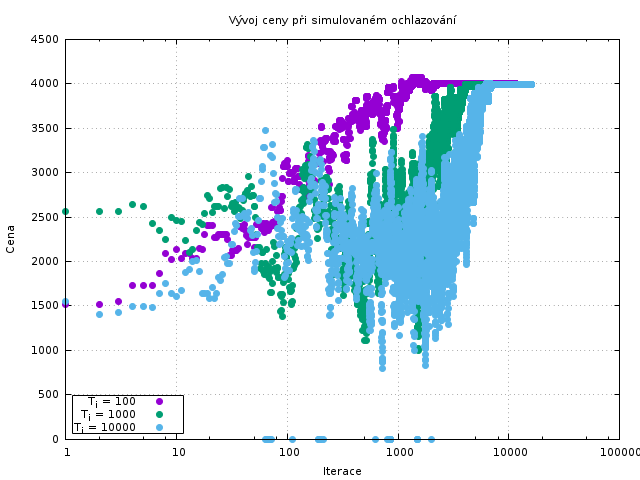
\includegraphics[width=0.8\textwidth]{../grafy/progress.png}
	\caption{Vývoj ceny při simulovaném ochlazování}
	\label{fig:progress}
\end{figure}

\subsection{Závislost na počáteční teplotě}
\label{sec:temp}

Na grafu \ref{fig:temp_init} můžeme pozorovat, že doba běhu roste logaritmicky se zvyšující se teplotou. Počáteční teplota totiž kromě pravděpodobnosti provedení tahu také ovlivní (stejně jako koeficient ochlazování a bod zamrznutí) počet iterací algoritmu. 

Z kostry algoritmu v sekci \ref{sec:kostra} vyplívá, že teplota klesá v průběhu výpočtu exponenciálně v závislosti na koeficientu ochlazování, z čehož vyplívá logaritmická závislost.

\begin{figure}[h!]
	\centering
    	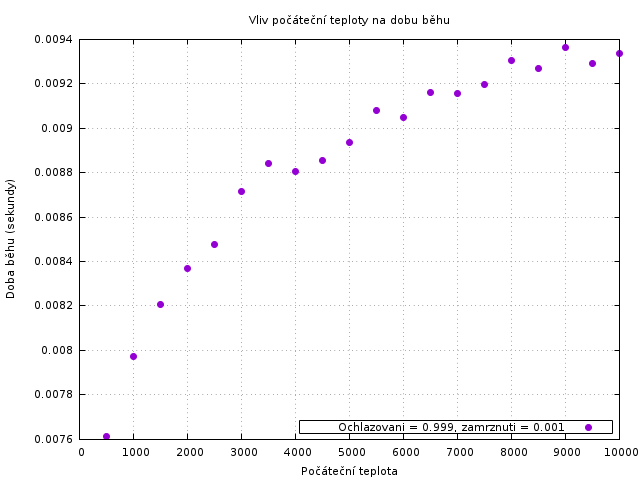
\includegraphics[width=0.8\textwidth]{../grafy/temp_init.png}
	\caption{Vliv počáteční teploty na dobu běhu}
	\label{fig:temp_init}
\end{figure}

Vliv počáteční teploty na relativní chybu je znázorněn na grafu \ref{fig:temp_init_e}. Z něj je patrné, že kvalita 
řešení se ustálí již při počáteční teplotě $T_i = 80$, a tedy nemá smysl volit větší hodnoty.

Graf \ref{fig:temp_init_e2} zobrazuje relativní chybu při počátečních teplotách ve větším rozsahu (stejném jako v grafu \ref{fig:temp_init}). Kvalita řešení se tedy nezmění ani pro vysoké počáteční teploty a relativní chyba se stále drží kolem hodnoty 0.02.

\begin{figure}[h!]
	\centering
    	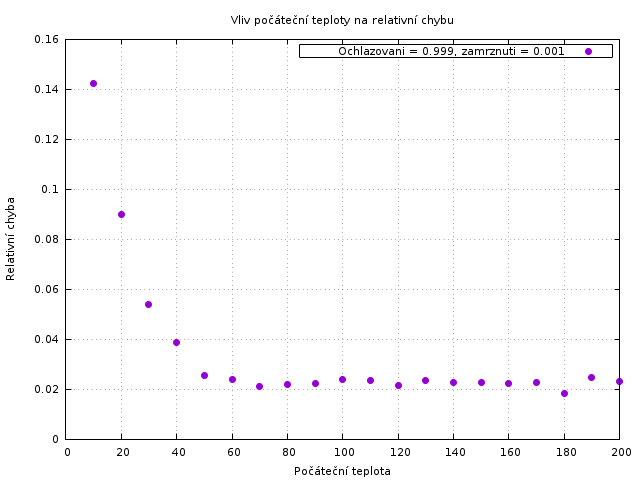
\includegraphics[width=0.8\textwidth]{../grafy/temp_init_e2.png}
	\caption{Vliv počáteční teploty na relativní chybu}
	\label{fig:temp_init_e}
\end{figure}

\begin{figure}[h!]
	\centering
    	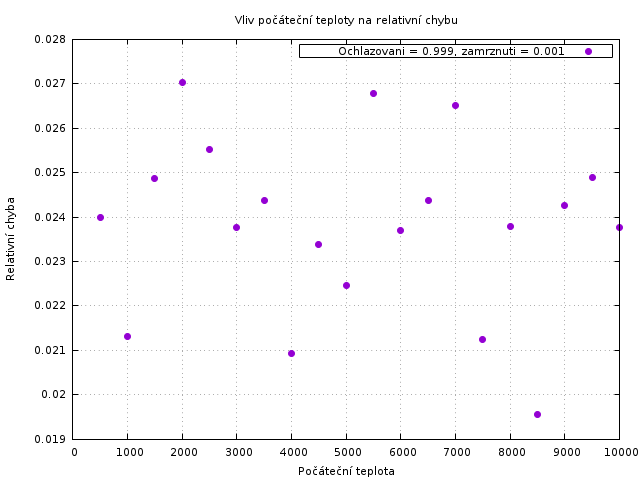
\includegraphics[width=0.8\textwidth]{../grafy/temp_init_e.png}
	\caption{Vliv počáteční teploty na relativní chybu (větší rozsah hodnot)}
	\label{fig:temp_init_e2}
\end{figure}

\subsection{Závislost na rychlosti ochlazování}

Pro další měření byla zvolena počáteční teplota $T_i = 500$. V sekci \ref{sec:temp} stačila k nalezení stejně kvalitního řešení i výrazně nižší teplota, zde však docházi ke změnám ostatních parametrů heuristiky.

Podle očekávání při pomalejším ochlazování roste doba běhu algoritmu (graf \ref{fig:cool}), neboť se teplota bodu zamrznutí přibližuje pomaleji.

\begin{figure}[h!]
	\centering
    	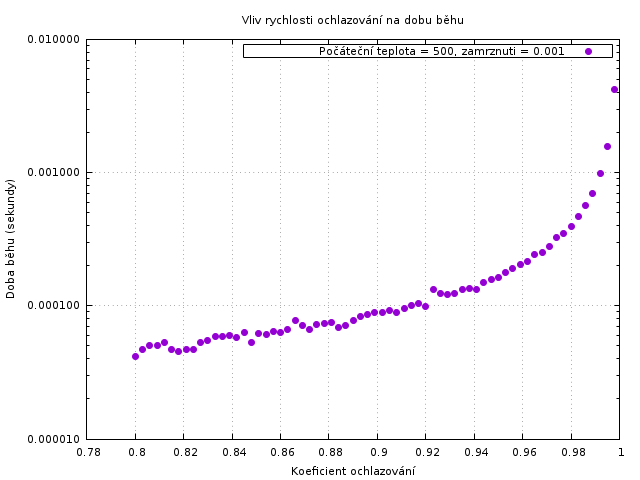
\includegraphics[width=0.8\textwidth]{../grafy/cool.png}
	\caption{Vliv rychlosti ochlazování na dobu běhu}
	\label{fig:cool}
\end{figure}

Z grafu \ref{fig:cool_e} je vidět, že relativní chyba s pomalejším ochlazováním klesá, což je opět přepokládané chování, neboť větší počet iteraci dovoluje prozkoumat větší počet tahů.

Narozdíl od závisloti na počáteční teplotě, kde k ustálení relativní chyby došlo poměrně rychle a růst doby běhu byl pomalý, má volba rychlosti ochlazování mnohem výraznější vliv na dobu běhu i chybu algoritmu. Je tedy otázka kolik výpočetního času jsme ochotni obětovat za kvalitnější řešení.

\begin{figure}[h!]
	\centering
    	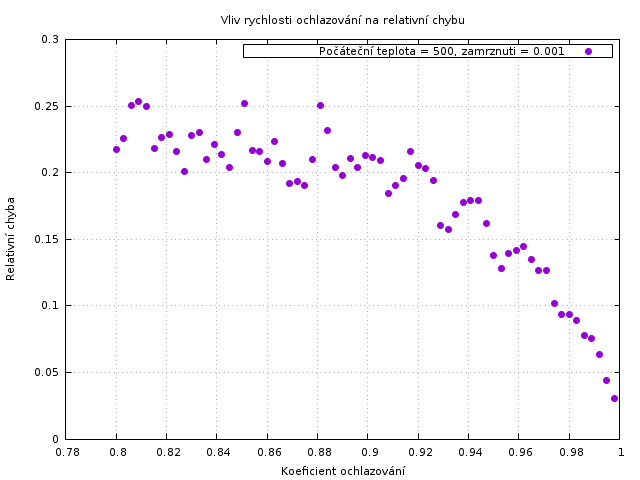
\includegraphics[width=0.8\textwidth]{../grafy/cool_e.png}
	\caption{Vliv rychlosti ochlazování na relativní chybu}
	\label{fig:cool_e}
\end{figure}

\subsection{Závislost na bodu zamrznutí}

Vliv bodu zamrznutí je podobý jako vliv počáteční teploty. Se zmenšujícím se bodem zamrznutí tedy roste počet iterací algoritmu a tím i doba běhu, jak můžeme pozorovat na grafu \ref{fig:frozen}.

\begin{figure}[h!]
	\centering
    	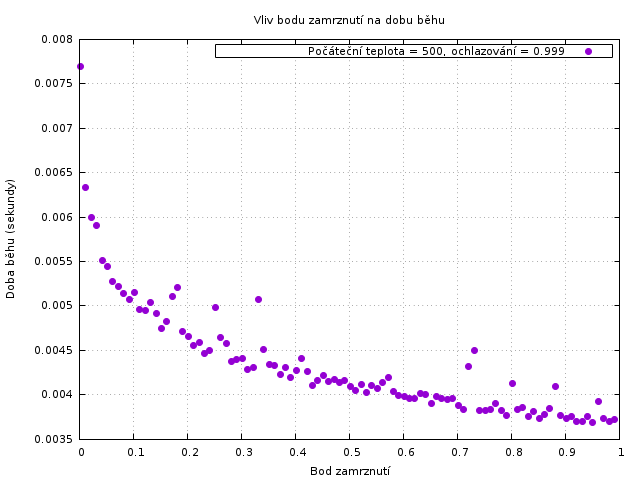
\includegraphics[width=0.8\textwidth]{../grafy/frozen.png}
	\caption{Vliv bodu zamrznutí na dobu běhu}
	\label{fig:frozen}
\end{figure}

Z grafu \ref{fig:frozen_e} vyplívá, že vliv bodu zamrznutí na chybu algoritmu žádný pozorovatelný vliv nemá. Je však možné, že by výsledky ovlivnil při změně dalších parametrů. 

\begin{figure}[h!]
	\centering
    	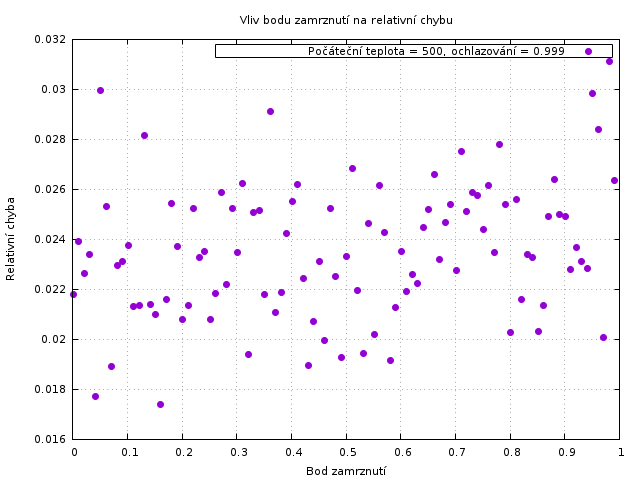
\includegraphics[width=0.8\textwidth]{../grafy/frozen_e.png}
	\caption{Vliv bodu zamrznutí na relativní chybu}
	\label{fig:frozen_e}
\end{figure}

\section{Závěr}

Heuristika je tedy podle očekávání poměrně citlivá na nastavení parametrů. Tato citlivost se projeví jak na času výpočtu tak na kvalitě nalezeného řešení.

Určit vhodnou hodnotu parametru se zdá být nejsnažší u počáteční teploty, neboť vliv na dobu běhu je malý a od určíté hodnoty již nelze zlepšit kvalitu řešení. 

Zvolit rychlost ochlazování je složitější, neboť nalézt kvalitnější řešení je výrazně časově náročnější. I zde lze předpokládat horní mez, nad kterou již kvalita řešení neporoste, přiblížit se této mezi však může být časově neúnosné. Záleželo by tedy na konkrétním využití algoritmu.

Žádný výrazný vliv bodu zamrznutí na chybu algoritmu se mi nepodařilo prokázat, při volbě tohoto parametru by tedy měl být zohledněn především jeho vliv na dobu běhu. Je však možné, že při jiných vstupních datech, případně při jiném nastavení ostatních parametrů by nějaká závislost vyšla najevo.

\bibliographystyle{csn690}
\bibliography{mybibliographyfile}

\end{document}
